\section{Un sistema prepago para Ángola}
En el anterior número hablamos de sistemas de prepago de manera genérica. En esta ocasión, se explica con mayor detalle un sistema de prepago para la realidad angolana.

\subsection{Descripción de los equipos que componen el sistema}
A continuacion se describen los equipos necesarios para el sistema que se propone (véase Figura \ref{fig:componentes})
\begin{enumerate}
\item El dispositivo de medida será un contador monofásico o trifásico con elemento de corte
integrado.
\item El sistema de comunicaciones estará basado en el PLC (Power Line
Communications): sistema de comunicación que emplea la red eléctrica para el intercambio de información entre equipos conectados a esta.
\item Se dispondrá de un elemento llamado concentrador que será el encargado de
gestionar la red formada por los contadores. Sus principales funciones serán: captar la información proveniente de los contadores y enviar las órdenes necesarias a los mismos para que su funcionamiento
sea el adecuado (cambio de tarifa, desactivación remota del relé, etc.).
\item Se dispondrá además del software de control PowerPLC que es el que permite de
forma básica gestionar todas las funciones del sistema.
\end{enumerate}

\begin{figure}[ht!]
\begin{center}
\begin{figurebox}
  \centering
    \begin{subfigure}{.2\textwidth}
  \centering
   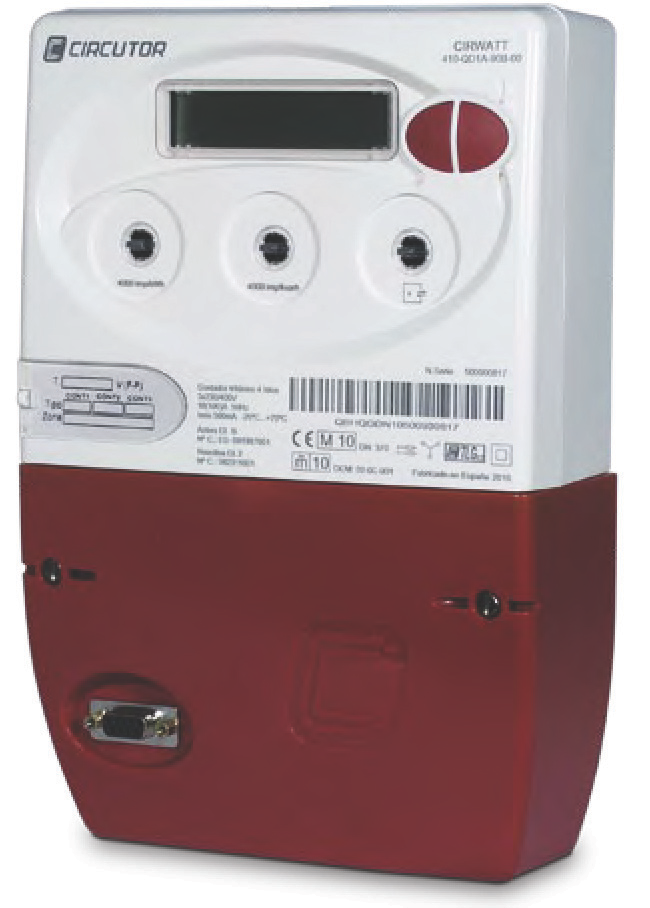
\includegraphics[height=50pt]{cirwat.png}
   \caption{Contador}
\end{subfigure}
 \begin{subfigure}{.2\textwidth}
  \centering
   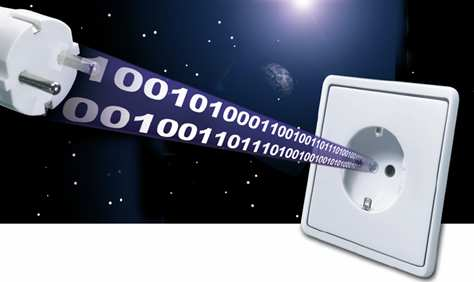
\includegraphics[height=50pt]{PLC.png}
   \caption{PLC}
\end{subfigure}
\begin{subfigure}{.2\textwidth}
\centering
  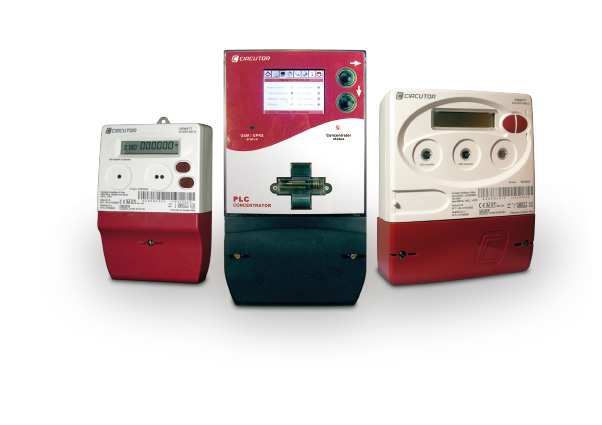
\includegraphics[height=50pt]{Concentrador.png}
  \caption{Concentrador}
 \end{subfigure}
 \begin{subfigure}{.2\textwidth}
  \centering
   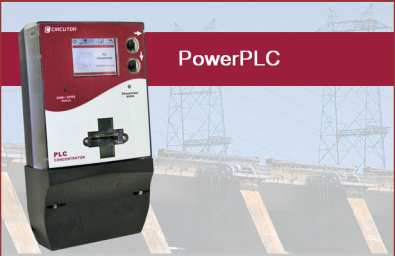
\includegraphics[height=50pt]{PowerPLC.png}
   \caption{Software}
\end{subfigure} \caption{Ejemplo de elementos de un sistema de prepago para Ángola.} \label{fig:componentes}
\end{figurebox}
\end{center}
\end{figure}

\subsection{Descripción del sistema}
\begin{itemize}
\item Existirán dos tipo de contratos para los usuarios finales:
\begin{itemize}
  \item Contrato básico, sólo tarifa 1. En el caso de que la energía provenga del
grupo electrógeno (tarifa 2), el contador desconectará el suministro con
la ayuda del elemento de corte interno.
 \item  Contrato extendido, tarifa 1 y tarifa 2. En el caso de que la energía
provenga del grupo electrógeno, el contador pasará a acumular la
energía en el registro de la tarifa 2.
\end{itemize}
\item El concentrador dispondrá de una entrada auxiliar a la que tenemos que aplicar
230 Vac para activarla, que le indicará de donde proviene la fuente de energía:
\begin{itemize}
\item Entrada auxiliar alimentada: la energía proviene del grupo generador.
\item Entrada auxiliar no alimentada: la energía proviene de la red pública.
\end{itemize}
\item  En los contadores tendremos configurado el tipo de contrato básico o
extendido, y en cuanto el concentrador detecte que se ha cambiado ha
 entrado en funcionamiento el grupo electrógeno, enviará un comando por la propia red a todos los contadores para ndicarles que pasaran a trabajar con la segunda tarifa aquellos contadores que
la tengan seleccionada desconectando el sistema los contadores con contrato básico.
\item El concentrador enviará la indicación de tarifa a los contadores de la siguiente
forma:
\begin{itemize}
\item Cada cinco minutos envía la los contadores un comando indicando cual
es la tarifa activa en función del estado de la entrada de selección de
tarifa.
\item  Enviará de forma inmediata el comando vía PLC de cambio de tarifa en
cuanto haya un cambio de estado en la entrada de selección de tarifa.
\end{itemize}
%\item Si el contador no recibe ningún comando de tarifa vía PLC durante 30 minutos,
%pasará de forma automática a la tarifa 1.
%\item Si el contado se apaga, al arrancar trabajará siempre con la tarifa 1 hasta que
%reciba el comando de mantenerse en esa tarifa o cambiar a la 2.
\item De forma remota desde el concentrador se podrá leer el consumo asociado a
cada una de las tarifas.
\end{itemize}

\section{Características del sistema de prepago}
En el contador se pueden configurar cuatro nuevos parámetros:
\begin{enumerate}
\item Tipo de contrato:
\begin{enumerate}
  \item Básico: Sólo tarifa 1.
  \item Extendido: Tarifa 1 y tarifa 2 (Generador).
\end{enumerate}
\item Modo de prepago:
\begin{enumerate}
   \item Prepago NO.
   \item Prepago SI.
\end{enumerate}
\item Energía correspondiente al prepago (expresada en kWh con un
  decimal: XXXX.X): es la cantidad de energía que queda en la cuenta
  de cada cliente, esta cuenta se recarga periódicamente en el punto
  de recarga autorizado y corresponde al saldo en función de cada una
  de las tarifas. La tarifa 2 será más cara ya que de su recaudación
  será la que permita la operación y mantenimiento del generador de
  emergencia.
\item Energía correspondiente a la pre-alarma (expresada en kWh con un
  decimal: XXXX.X): este valor puede ser programado a voluntad del
  gestor del sistema de manera que facilite una señal de alarma para
  advertir a los clientes que su saldo energético está próximo a
  finalizar por lo que es necesaria una nueva recarga. En caso de que
  el registro de energía prepago llegue a 0, en ese momento el
  software enviará automáticamente al contador a través del
  concentrador la orden de apertura del relé de desconexión dejando
  fuera del sistema al cliente hasta que se efectúe una recarga de
  saldo.
\end{enumerate}

\section{Ejemplo de aplicación: Sistema Multitarifa en Condominios}

El mejor ejemplo donde podemos introducir este tipo de tecnología es
en condominios donde existe un gestor (que será el propietario del
condominio) que tiene contratado un suministro eléctrico a la empresa
de distribución pero que como existen cortes de suministro quiere
garantizar a los usuarios un servicio eléctrico 24/24 para lo que
instala un generador eléctrico de emergencia.

En estos casos instalaríamos un sistema formado por contadores
inteligentes (monofásicos o trifásicos en función de las necesidades
energéticas de cada uno de los clientes del condominio) de medida
directa con capacidad de cortar el servicio de manera automática
comunicados entre sí por medio de la red eléctrica gracias a un
concentrador. Como describimos anteriormente, el sistema PLC es capaz
de permitir la comunicación entre los distintos elementos a través de
la red eléctrica por lo que no será necesaria la instalación de nuevas
redes de comunicación. Podemos instalar el concentrador en una zona
cercana al edificio administrativo del condominio de manera que
podamos comunicarlo con el computador con un cable de red y gracias a
esta tecnología PLC llegaremos a comunicarnos con todos los puntos del
condominio donde llegue la línea eléctrica. Cabe destacar que en caso
de que existan varios transformadores habrá que conectar un
concentrador por cada transformador ya que la tecnología PLC no es
capaz de salvar los trafos de aislamiento ni los bobinados entre baja
y media tensión ya que requiere de la continuidad del cable eléctrico.




El software de control integra la posibilidad de discriminar la
energía procedente de la red pública y la procedente del sistema de
emergencia de manera que los usuarios que deseen tener garantizada
energía ininterrumpida colaboran en la operación y mantenimiento de
los generadores (existen dos registros de contaje por contador a los
que se les aplica una tarifa diferente en función de la fuente de
procedencia). Los usuarios que no deseen poseer servicio de emergencia
serán desconectados de la red automáticamente en el momento que exista
un corte de suministro de la red pública. Además de esta función
automática, el gestor dispondrá de información en el programa de
control que le permita optar por varias posibilidades de facturación a
los usuarios, por facturas a mes vencido o por sistema prepago (cada
usuario cargará desde el centro de control administrado por el gestor
del condominio un saldo a su cuenta que será descontado a medida que
exista un consumo sea con una tarifa o con dos, cuando se alcance un
\% del total configurado a voluntad del gestor aparecerá una alarma
para que advirtamos al usuario de que necesita recargar su saldo para
no sufrir una interrupción del suministro eléctrico).


Estos sistemas de facturación favorecen tanto al gestor del centro
residencial como a los residentes ya que por un lado el gestor se
asegura de que todos sus clientes abonarán de manera solidaria y
proporcional a su consumo la energía empleada, sea procedente de la
red pública como del sistema de emergencia. De esta manera se puede
realizar una previsión de los costes de gestión y mantenimiento de
todos los servicios conociendo el coste anual y beneficios del
sistema. Por otro lado los residentes se beneficiarán de poseer un
sistema eléctrico bien gestionado y organizado de manera que pagarán
exclusivamente la energía que consuman por lo que se premiará el
ahorro energético y por otro lado podrán exigir al propietario del
centro residencial una calidad mínima en el suministro de la energía
ya que se está pagando por el servicio.
 
     

%\begin{wrapfigure}{r}{0.5\textwidth} 
%\vspace{-1cm}
%  \begin{figurebox}
%    \vspace{0.1cm}
%  \centering
%  \includegraphics[width=\textwidth]{TuberiaMolecor.jpg}
%  \caption{Tuberías  TOM\textcopyright \,  PVC-0 de Molecor.}
%  \label{fig:1}
%\end{figurebox}
%\end{wrapfigure}

%\vspace{3.75cm} 
%\noindent
%
\includegraphics[width=\textwidth,scale=0.5]{pubmm.png}
\newpage
%%% Local Variables: 
%%% mode: latex
%%% TeX-master: "novedades"
%%% End: 


